\documentclass[11pt]{ctexart} % 10pt即5号字体
\linespread{1.2} % 行距为1.2
\usepackage{url}  % 使用宏包url提供超链接
\usepackage[top=2cm, bottom=3cm, left=3cm, right=3cm]{geometry}  % 使用geometry来控制页面布局
\usepackage{graphicx}
\title{\centering \LARGE{LZW 文档说明}\\% Title
} % Subtitle
\author{\textsc {陈李锋 14通信 2014081025 } }

%----------------------------------------------------------------------------------------

\begin{document}

\maketitle % Print the title section

\subsubsection*{\raggedleft{操作系统和编译器说明}}
\paragraph{}
\begin{itemize}
\item[-] 操作系统: ubuntu 16.04lts
\item[-] 编译器: gcc
\item[-] 输入文件文件类型:html
\end{itemize}

\subsubsection*{\raggedleft{lzw压缩算法简单说明}}
重要对象说明 :
\begin{itemize} 
\item 字符(character):最基础的数据元素,在文本文件中就是一个字节 
\item 字符串(string):由几个连续的字符组成
\item 码长(codeLength):取12位
\item 字典容量(dictionarySize): 取 2的12次幂 4096个
\item 编码压缩(compress):编码依据是先将数据的个别单一字符ascii码先创建成一个字符串编码表,再分别给予编号,
在随后的编(解)码过程,字符串编码表会随着字符串键入而逐渐扩大
\item 解码译码(decompress):解码依据是将压缩数据与原先字符串编码表对照,并将对应的字符放于一个暂存队列中,
依序将压缩数据读入,若为重复数据保存于队列中,若不为重复数据,则扩充一个新的码置于字符串编码表中。
\item 文档格式: 需要输入的是html英文文档,压缩后的为.lzw格式文件
\end{itemize}

\subsubsection*{\raggedleft{操作}}
\begin{itemize} 
\item[] 编译: gcc lzw.c -o lzw
\item[] 压缩文件: ./lzw c test.html 
\item[] 解压文件: ./lzw d test.pdf.lzw 
\end{itemize}

\subsubsection*{\raggedleft{结果演示}}
\begin{itemize}
\item[] 压缩: 把501k大小的test.html压缩成112k test.html.lzw

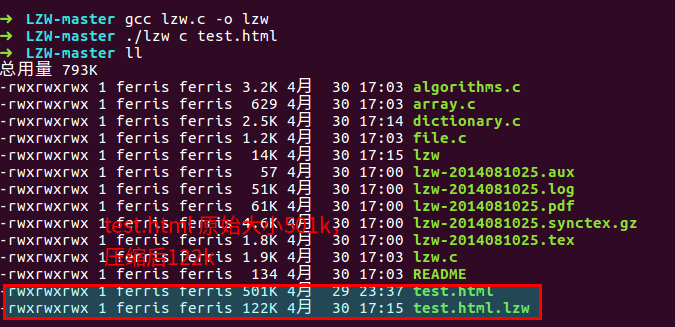
\includegraphics[width=5in]{pic001}

\item[] 解压:由112k test.html.lzw解压成原来的501k大小的test.html

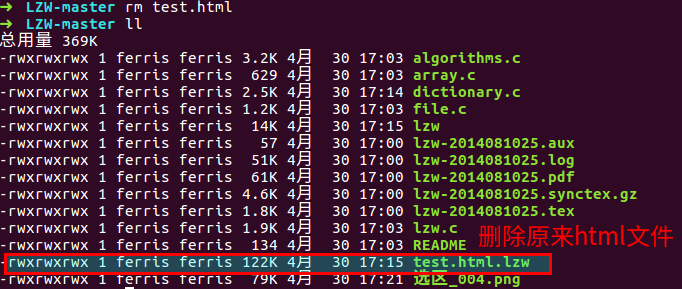
\includegraphics[width=5in]{pic002}

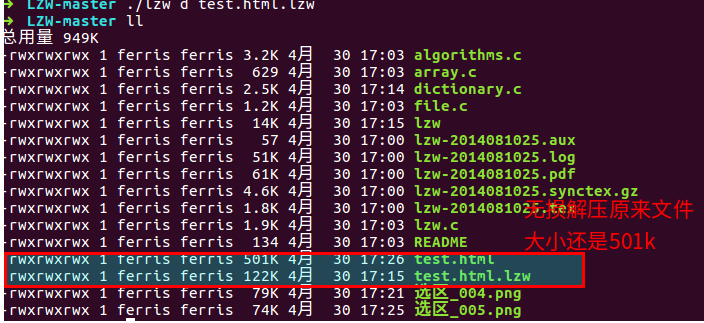
\includegraphics[width=5in]{pic003}
\end{itemize}
由此可以看出,代码实现了压缩的效果,并且压缩效果也不错。

\end{document}